\documentclass[a4paper, 12pt]{article}
\usepackage[T1]{fontenc}
\usepackage{lmodern}
\usepackage{color}
\usepackage{amsfonts}
\usepackage{epstopdf}
\usepackage{matlab}
%\documentclass{book}
\usepackage{blindtext}
\usepackage{hyperref}
\usepackage[brazil]{babel}
\usepackage{amssymb}
\usepackage[utf8]{inputenc}
\usepackage{amsmath}
\usepackage{indentfirst}
\usepackage{graphicx}
\usepackage{multicol,lipsum}
\usepackage[a4paper, top=3cm, left=3cm, bottom=3cm, right=3cm]{geometry}
\usepackage{setspace}
\usepackage{multirow}
\usepackage{float}
\usepackage[table]{xcolor}
%\usepackage{pdflscape}
\usepackage[DIV=15]{typearea}
\usepackage[nottoc]{tocbibind}
\usepackage[sort,numbers]{natbib}
%\usepackage{cite}

\documentclass[letterpaper]{article}
% bib pack %%%%%%%%%%%%%%%%%%%%%%%%%%%%%%%%%%%%%%%%%%%%%%%%%%%%%%%%%%%%%%%%%%%%%
\usepackage[utf8]{inputenc}
\usepackage{geometry}
    \geometry{left=3cm,right=2cm,top=2cm,bottom=2cm}
%
\usepackage[spanish]{babel}
%
\usepackage[fixlanguage]{babelbib}
    \bibliographystyle{babunsrt}
%
\usepackage{url}

\begin{document}
%\maketitle

\begin{titlepage}
	\begin{center}
		

\vspace{10pt}
%\begin{figure}[!ht]
%\centering
%
\includegraphics{puc-rio-logo.png}

%\end{figure}
\begin{figure}[!ht]
\centering

\includegraphics{images/puc-rio-logo.png}
\end{figure}
\huge{Laboratório de Controles e Servomecanismos}
        \vspace{70pt}
        
		\textbf{ENG1418}
		\textbf{\large{\\ }}
		
		\vspace{30pt}
		\textbf{\small{\\PROJETO 4}}
		\vspace{65pt}
		
	\end{center}
	
	\begin{flushleft}
		\begin{tabbing}
			Aluno(a)\qquad\qquad\=\>Gabriel Mota Botelho - 1620628\\
			\>Paloma Fernanda Loureiro Sette - 1621595\\
			
			Professor(a)\>Vivian Suzano Medeiros\\
	\end{tabbing}
		  
	\end{flushleft}
	\begin{center}
		%\vspace{\fill}
		\vspace{80pt}
		Rio de Janeiro, 30 de Maio de 2022
	\end{center}
\end{titlepage}
%%%%%%%%%%%%%%%%%%%%%%%%%%%%%%%%%%%%%%%%%%%%%%%%%%%%%%%%%%%
\newpage
\tableofcontents
\thispagestyle{empty}

\newpage
\pagenumbering{arabic}

\newpage

%\newcommand{\listequationsname}{Lista de Equações}
%\newlistof{myequations}{equ}{\listequationsname}
%\newcommand{\myequations}[1]{%
%\addcontentsline{equ}{myequations}{\protect\numberline{\theequation}#1}\par}

%\listofmyequations
\newpage


\newpage

\listoffigures
\thispagestyle{empty}

\newpage
%%%%%%%%%%%%%%%%%%%%%%%%%%%%%%%%%%%%%%%%%%%%%%%%%%%%%%%%%
%%%%%%%%%%%%%%%%%%%%%%%%%%%%%%%%%%%%%%%%%%%%%%%%%%%
\section{Motivação}
O objetivo deste trabalho é consolidar os conceitos de análise de sistemas em relação a estabilidade, controlabilidade e observabilidade, utilizando o MATLAB/Scilab.

\section{Introdução}
Para que problemas reais possam ser interpretados e estudados a fim de se obter um resultado, precisa-se que as informações referentes
ao problema sejam analisadas e processadas por várias teorias já estudadas ao longo do tempo. Essas teorias funcionam como ferramentas do estudo, e, a partir delas, é
possível que um fenômeno físico seja descrito por equações. 

Nosso intuito é analisar o sistema não-linearizado do pêndulo
invertido perante as incertezas significativas inerentes a ele. Posteriormente, em outro problema, analisaremos o circuito RLC.



\section{Problema 1}
Devemos, a princípio, considerar o seguinte sistema, que representa um pêndulo invertido montado em um carro motorizado.
Consideremos também que a massa da haste está concentrada no topo e o centro de gravidade é o centro da bola do pêndulo. Para esse caso, o momento de inércia do pêndulo sobre seu centro de gravidade é pequeno e podempos assumir momento de inércia I = 0.

\begin{figure}[H]
\centering
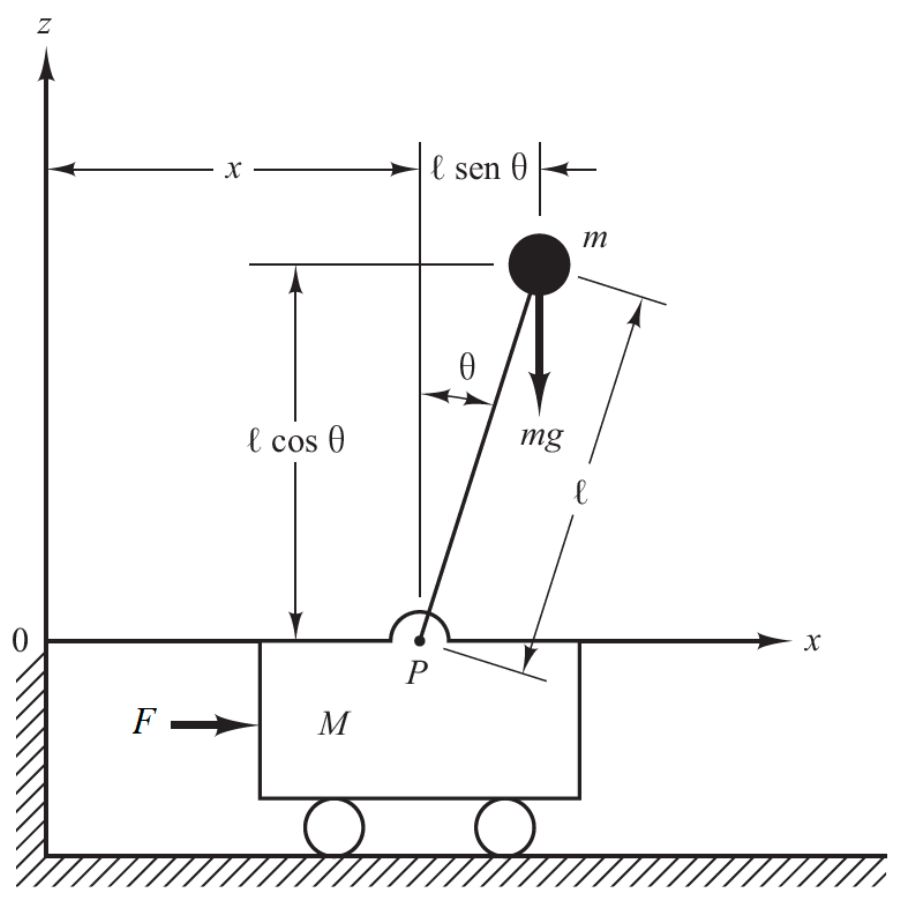
\includegraphics[scale = 0.7]{images/sistema-prob1.png}
\label{filtro1}
\caption{Sistema do problema 1}
\end{figure}



\subsection{Modelagem}

\subsubsection{Espaço de Estados}
A partir deste subtópico, modelaremos o sistema em espaço de estados, considerando que a entrada é a força \textit{F} aplicada ao carrinho e a saída é o ângulo $\theta$ de deslocamento do pêndulo.

considerando $\theta$ como o ângulo de deslocamento da haste e as coordenadas $(x, y)$ como o centro de gravidade da haste do pêndulo como $X_{G}$, $Y_{G}$. Então,

\begin{equation}\label{eq:cd}
    X_{G} = x + lsen\theta
\end{equation}


\begin{equation}\label{eq:cd}
    Y_{G} = lcos\theta
\end{equation}

A soma das forças resultantes de rotação da haste do pêndulo em torno de seu centro de gravidade pode ser
descrito em \ref{eq:movi_01}, onde $F_{gx}$ e $F_{gy}$ são as componentes da força peso da haste.

\begin{equation}\label{eq:movi_01}
    I\frac{d^2\theta}{dt^2} = F_{gy}lsen\theta - F_{gx}lcos\theta
\end{equation}

As equações que descrevem o \textbf{movimento horizontal} e o \textbf{movimento vertical} do centro de gravidade da haste do pêndulo e o \textbf{movimento horizontal do carrinho} estão descritas em, respectivamente, \ref{eq:movi_H}, \ref{movi_V} e \ref{eq:movi_HCARRO}.

\begin{equation}\label{eq:movi_H}
    \frac{md^2}{dt^2}(x + l sen\theta) = F_{gx}
\end{equation}



\begin{equation}\label{movi_V}
    \frac{md^2}{dt^2}(lcos\theta) = F_{gy} - mg
\end{equation}



\begin{equation}\label{eq:movi_HCARRO}
    M\frac{d^2x}{dt^2} = F - F_{gx}
\end{equation}

%sentheta = theta ; costheta = 1; theta*theta^2 = 0


Como devemos manter o pêndulo invertido na vertical, supõe-se que $\theta(t)$ e $\frac{d\theta}{dt}$ são
pequenos tais que $sen\theta = \theta$, $cos\theta = 1$. Logo,


\begin{equation}\label{eq:movi_3}
    I\frac{d^2\theta}{dt^2} = F_{gy}l\theta - F_{gx}l
\end{equation}

\begin{equation}\label{eq:movi_4}
    m(\frac{d^2x}{dt^2} + l\frac{d^2\theta}{dt^2}) = F_{gx}
\end{equation}

\begin{equation}\label{eq:movi_5}
    0 = F_{gy} - mg
\end{equation}

Com as Equações \ref{eq:movi_HCARRO} e \ref{eq:movi_4}, temos,

\begin{equation}\label{eq:movi_6}
    (M + m)\frac{d^2x}{dt^2} + ml\frac{d^2\theta}{dt^2} = F
\end{equation}

Com as Equações \ref{eq:movi_3}, \ref{eq:movi_4} e \ref{eq:movi_5}, temos,

\begin{equation}\label{eq:cd}
    I\frac{d^2\theta}{dt^2} = mgl\theta - l(m\frac{d^2x}{dt^2} + ml\frac{d^2\theta}{dt^2})
\end{equation}

\begin{equation}\label{eq:cd}
    (I + ml^2)\frac{d^2\theta}{dt^2} ml\frac{d^2x}{dt^2} = mgl\theta
\end{equation}

Como I = 0,

\begin{equation}\label{eq:movi_10}
    ml^2\frac{d^2\theta}{dt^2} + ml\frac{d^2x}{dt^2} = mgl\theta
\end{equation}

Enfim, as equações finais que descrevem o sistema estão descritas em \ref{eq:movi_11} e \ref{eq:movi_13}

\begin{equation}\label{eq:movi_11}
    \fbox {\huge$ (M + m)\frac{d^2x}{dt^2} + ml\frac{d^2\theta}{dt^2} = F$}
\end{equation}

\begin{equation}\label{eq:movi_13}
    \fbox {\huge $  l\frac{d^2\theta}{dt^2} + \frac{d^2x}{dt^2} = g\theta $}
\end{equation}

Definindo as variáveis de estado como,

\begin{equation}\label{eq:movi_12}
   x_{1} = \theta
\end{equation}

\begin{equation}\label{eq:movi_12}
    x_{2} = \frac{d\theta}{dt}
\end{equation}

\begin{equation}\label{eq:movi_12}
   x_{3} = x
\end{equation}

\begin{equation}\label{eq:movi_12}
   x_{4} = \frac{dx}{dt}
\end{equation}

Logo, pela definição de variável de estado, temos,

\begin{equation}\label{eq:movi_12}
   \frac{dx_{1}}{dt} = x_{2}
\end{equation}

\begin{equation}\label{eq:movi_12}
    \frac{dx_{2}}{dt} = \frac{M + m}{Ml}gx_{1} - \frac{1}{Ml}F
\end{equation}

\begin{equation}\label{eq:movi_12}
   \frac{dx_{3}}{dt} = x_{4}
\end{equation}

\begin{equation}\label{eq:movi_12}
   \frac{dx_{4}}{dt} = -\frac{m}{M}gx_{1} + \frac{1}{M}F 
\end{equation}

Com isto, geramos a representação de espaço de estados do sistema pêndulo invertido

\begin{equation}\label{eq:movi_12}
\begin{bmatrix}
\frac{dx_{1}}{dt}\\
\frac{dx_{2}}{dt}\\
\frac{dx_{3}}{dt}\\
\frac{dx_{4}}{dt}\\
\end{bmatrix}
=
\begin{bmatrix}
0 & 1 & 0 & 0\\
\frac{M + m}{Ml}g & 0 & 0 & 0\\
0 & 0 & 0 & 1\\
-\frac{m}{M}g & 0 & 0 & 0\\
\end{bmatrix}
\begin{bmatrix}
x_{1} \\
x_{2} \\
x_{3}\\
x_{4} \\
\end{bmatrix}
+
\begin{bmatrix}
0 \\
-\frac{1}{Ml} \\
0\\
\frac{1}{M} \\
\end{bmatrix}
F
\end{equation}

\begin{equation}\label{eq:movi_12}
\begin{bmatrix}
y_{1}\\
y_{2}\\
\end{bmatrix}
=
\begin{bmatrix}
1 & 0 & 0 & 0\\
0 & 0 & 1 & 0\\
\end{bmatrix}
\begin{bmatrix}
x_{1} \\
x_{2} \\
x_{3}\\
x_{4} \\
\end{bmatrix}
\end{equation}

\subsubsection{Função de Transferência}
A função de transferência irá escrever as equações de movimento como uma função da saída para a entrada, i.e., $\frac{Y(s)}{U(s)}$ com $Y(s)$ sendo a saída e $U(s)$ sendo a entrada. Para nosso sistema, teremos duas funções de transferência, uma em que iremos traduzir a entrada $u$ para a saída do ângulo $\theta$ e outra para traduzir a entrada $u$ para a saída $x$.

A transformada de Laplace é uma ferramenta vital para a resolução de equações diferenciais e para descrevermos funções de transferência e, ainda que não entremos em detalhes a respeito desta ferramenta, é recomendável que entendamos sua finalidade.

Vale a pena notarmos que há uma transformação a ser feita entre a representação de espaço de estados e uma função de transferência.

\paragraph{Função de Transferência de Ângulo}:\\

\>Determinaremos a função de transferência para a entrada $u$ e para o ângulo $\theta$, ou seja,

\begin{equation}\label{eq:transf_func_model}
    \frac{\Theta(s)}{U(s)}
\end{equation}

Portanto, tomaremos a transfomada de Laplace das equações de movimento calculadas anteriormente e resolveremos para $\theta$. 

Temos nossas equações de movimento definidas em (\ref{eq:movi_11}) e (\ref{eq:movi_13}). Portanto, teremos as respectivas transformadas de Laplace:

\begin{equation}\label{eq:laplace_transform}
    U(s)-bX(s)s = (M+m)X(s)s^2+ml\Theta(s)s^2\\
\end{equation}

\begin{tabbing}
    \qquad\qquad\=\> onde,\\
    \\\qquad\qquad\qquad\=\> - $U(s)$ refere-se à força horizontal aplicada ao carro;\\
    \\\qquad\qquad\qquad\=\> - $b$ refere-se ao coeficiente de atrito.\\
        
\end{tabbing}

\\e, por fim, a transformada de Laplace de (\ref{eq:movi_13}):

\begin{equation}\label{eq:laplace_transform2}
    g\Theta(s)=X(s)s^2+l\Theta(s)s^2
\end{equation}

\\Podemos reescrever a equação \ref{eq:laplace_transform2} para substituir $X(s)$ na equação \ref{eq:laplace_transform}, nos permitindo relacionar $\Theta(s)$ diretamente a $U(s)$. Portanto, teremos:

\begin{equation}\label{eq:substit_transform_laplace1}
    X(s) = (\frac{g}{s^2}-l)\Theta(s)
\end{equation}

Então, substituindo \ref{eq:substit_transform_laplace1} em \ref{eq:laplace_transform}:

\begin{equation}
    U(s) = (M+m)X(s)s^2+bX(s)s+ml\Theta(s)s^2
\end{equation}
\begin{equation}
    U(s) = (M+m)(\frac{g}{s^2}-l)\Theta(s)s^2+bX(s)s+ml\Theta(s)s^2
\end{equation}

Podemos simplificar para:

\begin{equation}
    U(s) = \Theta(s)\frac{-lMs^3-bls^2+g(M+m)s+bg}{s}
\end{equation}

Que agora pode ser escrita como nossa função de transferência:

\begin{equation}
    \frac{\Theta(s)}{U(s)} = \frac{s}{-lM-bls^2+g(M+m)s+bg}
\end{equation}
\begin{equation}\label{eq:tranfer_func_angle}
    \frac{\Theta(s)}{U(s)} = \frac{\frac{-1}{lM}s}{s^3+\dfrac{b}{M}s^2-\frac{g(M+m)}{lM}s-\frac{bg}{lM}}
\end{equation}

\paragraph{Função de Transferência de Posição}:\\

\> Os mesmos passos anteriores serão tomados para obter a função de transferência de posição. Já temos as transformadas de Laplace, portanto, da equação \ref{eq:laplace_transform2}, teremos:

\begin{equation}\label{eq:eq_transf-posi1}
    \Theta(s)=X(s)\frac{s^2}{g-ls^2}
\end{equation}


Colocando \ref{eq:eq_transf-posi1} em \ref{eq:laplace_transform} para substituir $\Theta(s)$:

\begin{equation}
    U(s)-bX(s)s = (M+m)X(s)s^2+\frac{mls^2}{g-ls^2}X(s)s^2\\
\end{equation}
\begin{equation}
    U(s) = X(s)((M+m)s^2+\frac{mls^4}{g-ls^2}+bs)\\
\end{equation}

Que pode ser simplificado para:

\begin{equation}
    U(s) = X(s)(\frac{-lMs^4-bls^3+g(M+m)s^2+bgs}{g-ls^2})\\
\end{equation}

Portanto, podemos reescrever e obter nossa função de transferência de posição como:

\begin{equation}
    \frac{X(s)}{U(s)} = X(s)\frac{g-ls^2}{-lMs^4-bls^3+g(M+m)s^2+bgs}\\
\end{equation}

\begin{equation}
    \frac{X(s)}{U(s)} = X(s)\frac{\frac{1}{M}s^2-\frac{g}{lM}}{s^4+\frac{b}{M}s^3-\frac{g(M+m)}{lM}s^2-\frac{bg}{lM}s}\\
\end{equation}

\subsection{Análise}
Para a análise de estabilidade assintótica, verifica-se os autovalores da matriz de estabilidade. Substituindo o valor das constantes, temos,


\begin{equation}
        det(Is - A) = 0
\end{equation}

\begin{equation}
\begin{bmatrix}
s & 0 & 0 & 0\\
0 & s & 0 & 0\\
0 & 0 & s & 0\\
0 & 0 & 0 & s\\
\end{bmatrix}
-
\begin{bmatrix}
0 & 1 & 0 & 0\\
6.54 & 0 & 0 & 0\\
0 & 0 & 0 & 1\\
-3.27 & 0 & 0 & 0\\
\end{bmatrix}
= 0
\end{equation}


\begin{equation}
     s_{1} = 2.55\\
     s_{2} = -2.55\\
     s_{3},s_{4} = 0\\
\end{equation}
Não é estável no sentido de Lyapunov pois a matriz de estado possui um autovalor no semi-plano a direita. Por este mesmo motivo, \textbf{o sistema não é BIBO-Estável}.

Para analisar a controlabilidade e observabilidade completa do sistema, primeiro desenvolve-se as matrizes de controlabilidade e observabilidade. Começando pela matriz de controlabilidade:

\begin{equation}
Co
=
\begin{bmatrix}
B & AB & A^2B & A^3B\\
\end{bmatrix}
\end{equation}

\begin{equation}
Co
=
\begin{bmatrix}
0 & -0.0167 & 0 & -0.1090\\
-0.0167 & 0 & -0.1090 & 0\\
0 & 0.0667 & 0 & 0.0545\\
0.0667 & 0 & 0.0545 & 0\\
\end{bmatrix}
\end{equation}

Agora, a matriz de observabilidade:

\begin{equation}
Ob
=
\begin{bmatrix}
C\\
CA\\
CA^2\\ 
CA^3\\
\end{bmatrix}
\end{equation}

\begin{equation}
Ob
=
\begin{bmatrix}
1.0 & 0 & 0 & 0\\
0 & 0 & 1.0 & 0\\
0 & 1.0 & 0 & 0\\
0 & 0 & 0 & 1.0\\
6.54 & 0 & 0 & 0\\
-3.27 & 0 & 0 & 0\\
0 & 6.54 & 0 & 0\\
0 & -3.27 & 0 & 0\\
\end{bmatrix}
\end{equation}

O sistema é \textbf{completamente controlável e observável}, pois o das duas matrizes posto é igual ao posto da matriz de estabilidade.



\subsection{Simulação em Malha Aberta}

Utilizando o modelo de espaço de estados obtido no item 1, simularemos o sistema através do MATLAB, considerando que nossa entrada é um degrau unitário.

\sloppy
\epstopdfsetup{outdir=./}
\graphicspath{ {./malhaaberta_images/} }

\matlabtitle{Malha aberta}

\begin{matlabcode}
clc
clear
close all

\end{matlabcode}

\matlabheading{Definição dos parâmetros designados:}

\begin{matlabcode}

m = 10.0;
M = 30.0;
l = 2.0;
g = 9.8;

\end{matlabcode}

\matlabheading{Matrizes para o modelo de Espaço de Estados:}

\begin{matlabcode}

A = [0 1 0 0 ; (M+m)*g/M*l 0 0 0 ; 0 0 0 1 ; (-m/M)*g 0 0 0];
B = [0 ; 1/M*l ; 0 ; -1/M];
C = [1 0 0 0 ; 0 0 1 0];
D = [0];

sys = ss(A,B,C,D);
lambda = eig(A);

\end{matlabcode}

\matlabheading{SIMULAÇÃO}

\begin{matlabcode}

opt = stepDataOptions('StepAmplitude',1)
\end{matlabcode}
\begin{matlaboutput}
opt = 
  step with properties:

      InputOffset: 0
    StepAmplitude: 1

\end{matlaboutput}
\begin{matlabcode}
[y,tout,x] = step(sys,opt);

figure()
subplot(1,2,1)
plot(tout,x) 
grid on;
title('Variáveis de estado')
xlabel('t [s]')
legend('x [m]','dx/dt [m/s]','theta [rad]','dtheta/dt [rad/s]')

subplot(1,2,2)
plot(tout,y)
grid on
title('Saída do sistema')
ylabel('theta [rad]')
xlabel('t[s]')

sgtitle('Resposta a um degrau unitário')
\end{matlabcode}


\begin{figure}[H]
\centering
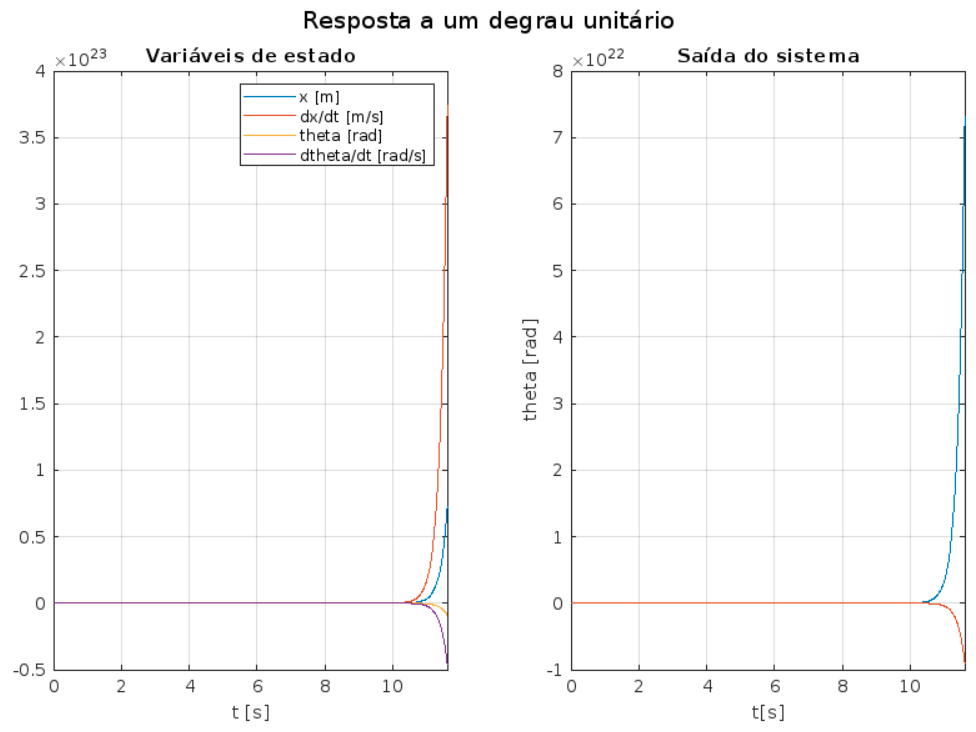
\includegraphics[scale = 0.4]{images/figure_0_matlab.png}
\label{filtro1}
\caption{Simualação em malha aberta}
\end{figure}

\subsection{Simulação em Malha Fechada}
Utilizando a função de transferência obtida anteriormente, $G(s)=\frac{\Theta(s)}{U(s)}$, em \ref{eq:tranfer_func_angle}, consideremos a seguinte malha de controle:

\begin{figure}[H]
\centering
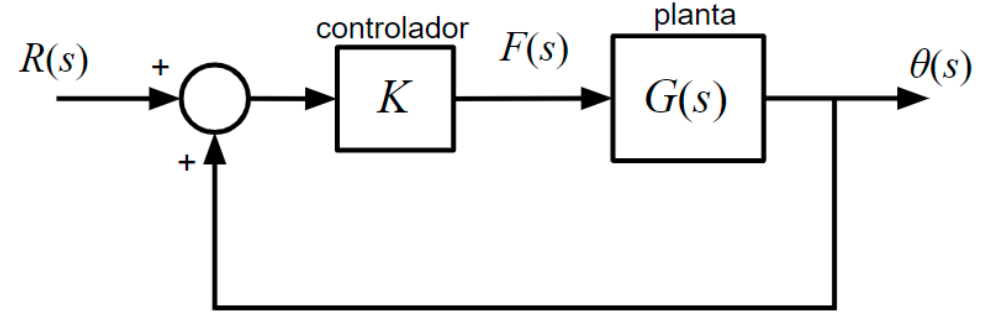
\includegraphics[scale = 0.7]{images/malha-controle.png}
\label{filtro1}
\caption{Malha de controle com realimentação}
\end{figure}

\sloppy
\epstopdfsetup{outdir=./}
\graphicspath{ {./malhafechada_images/} }

\matlabtitle{Malha fechada}

\matlabheadingtwo{Definição dos parâmetros designados}

\begin{matlabcode}
m = 10.0;
M = 30.0;
l = 2.0;
g = 9.8;

b = 0.1; %coeficiente de atrito arbitrário

f = g*(M+m)
\end{matlabcode}
\begin{matlaboutput}
f = 392
\end{matlaboutput}

\matlabheadingtwo{Gerando a função de transferência}

\begin{matlabcode}
Theta = -1/l*M;
U = [1 b/M -g*(M+m)/l*M -b*g/l*M];
G = tf(Theta, U)
\end{matlabcode}
\begin{matlaboutput}
G =
 
                 -15
  ----------------------------------
  s^3 + 0.003333 s^2 - 5880 s - 14.7
 
Continuous-time transfer function.
\end{matlaboutput}

\matlabheadingtwo{Para K \textless{} (M+m)g}

\begin{matlabcode}
syms s

%K < 392

K1 = 100;
Theta1 = Theta;
U1 = [1 b/M -K1/l*M -b*g/l*M];
G1 = tf(Theta1, U1)
\end{matlabcode}
\begin{matlaboutput}
G1 =
 
                 -15
  ----------------------------------
  s^3 + 0.003333 s^2 - 1500 s - 14.7
 
Continuous-time transfer function.
\end{matlaboutput}
\begin{matlabcode}
pole(G1);
\end{matlabcode}

\matlabheadingtwo{Para K = (M+m)g}

\begin{matlabcode}
%K = 392

K2 = f;
Theta2 = Theta;
U2 = [1 b/M -K2/l*M -b*g/l*M];
G2 = tf(Theta2, U2)
\end{matlabcode}
\begin{matlaboutput}
G2 =
 
                 -15
  ----------------------------------
  s^3 + 0.003333 s^2 - 5880 s - 14.7
 
Continuous-time transfer function.
\end{matlaboutput}
\begin{matlabcode}
pole(G2);
\end{matlabcode}

\matlabheadingtwo{Para K \textgreater{} (M+m)g}

\begin{matlabcode}
%K > 392

K3 = 500;
Theta3 = Theta;
U3 = [1 b/M -K3/l*M -b*g/l*M];
G3 = tf(Theta3, U3)
\end{matlabcode}
\begin{matlaboutput}
G3 =
 
                 -15
  ----------------------------------
  s^3 + 0.003333 s^2 - 7500 s - 14.7
 
Continuous-time transfer function.
\end{matlaboutput}
\begin{matlabcode}
pole(G3);
\end{matlabcode}

\matlabheadingtwo{SIMULAÇÃO}

\begin{matlabcode}
opt = stepDataOptions('stepAmplitude', 1);

[y1, tout1] = step(G1, opt);
figure()
subplot(1, 3, 1)
plot(tout1, y1); grid on
title('K < (m+M)g')
xlabel('t [s]')
legend('theta [rad]')

[y2, tout2] = step(G2, opt);
%figure()
subplot(1, 3, 2)
plot(tout2, y2); grid on
title('K = (m+M)g')
xlabel('t [s]')
legend('theta [rad]')

[y3, tout3] = step(G3, opt);
%figure()
subplot(1, 3, 3)
plot(tout3, y3); grid on
title('K > (m+M)g')
xlabel('t [s]')
legend('theta [rad]')

sgtitle('Resposta a um degrau unitário')
\end{matlabcode}

\begin{figure}[H]
\centering
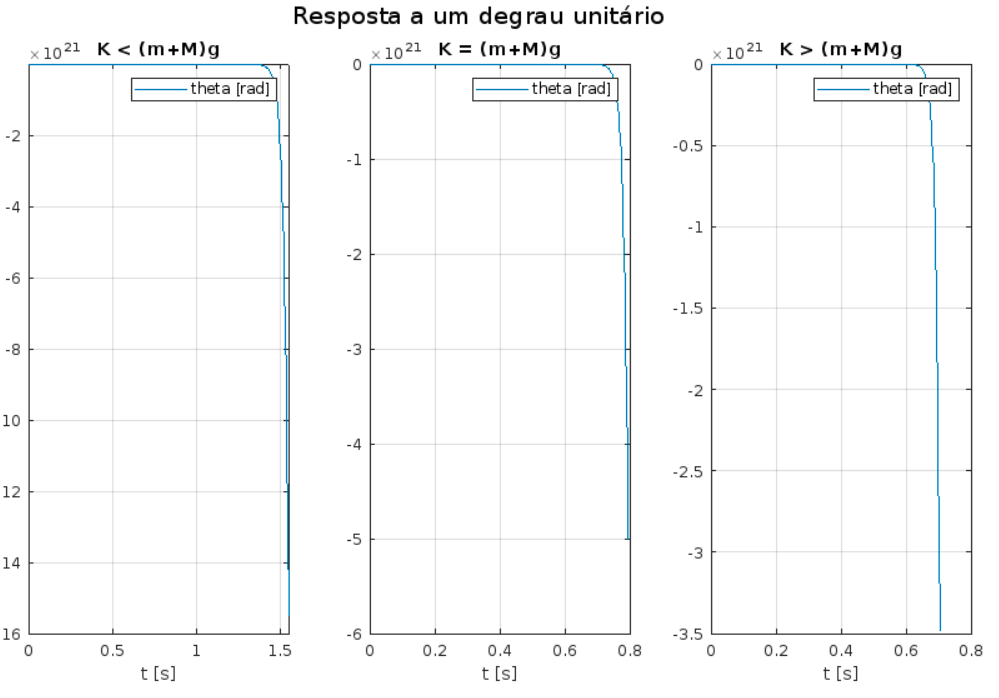
\includegraphics[scale = 0.4]{images/simulacao-malha-fechada.png}
\label{filtro1}
\caption{Simulação em malha fechada}
\end{figure}

\section{Problema 2}

Neste problema, nosso objetivo é analisar o circuito elétrico abaixo:

\begin{figure}[H]
\centering
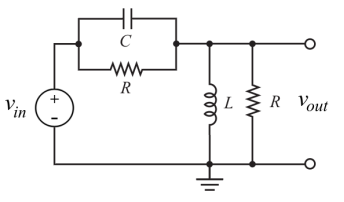
\includegraphics[scale = 0.7]{images/CIRCUITO_PROBLEMA-02.png}
\label{filtro1}
\caption{Sistema do problema 2}
\end{figure}

\subsection{Modelagem}
Para esse sistema, primeiro montamos as equações fisicas que regem o circuito RLC usando KCL e KVL. Já que o resistor está em paralelo com o capacitor, a tensão sobre os dois é igual. O mesmo pode se dizer para o resistor em paralelo com o indutor. Logo temos:

\begin{equation}\label{eq:circ 1}
    V - V_{R_{1}} - V_{L} = 0
\end{equation}

\begin{equation}\label{eq:circ 1}
    i_{R_{1}} + i_{C} - i_{L} - i_{R_{2}} = 0
\end{equation}

Tendo em vista que,

\begin{equation}\label{eq:circ 1}
    V_{R} = Ri_{r}
\end{equation}

\begin{equation}\label{eq:circ 1}
    V_{C} = \frac{1}{C}Q_{C}(t)
\end{equation}

\begin{equation}\label{eq:circ 1}
    V_{L} = L\frac{di_{L}(t)}{dt}
\end{equation}

Temos,

\begin{equation}\label{eq:circ 1}
    V - Ri_{r} - L\frac{di_{L}(t)}{dt} = 0
\end{equation}





\section{Conclusão}
\paragraph{}
Este trabalho propôs identificar a equação dinâmica dos sistemas sugeridos (pêndulo invertido e circuito RLC), objetivando a obtenção das funções de transferência e as respectivas equações de estados para posteriormente realizar a análise de estabilidade em malha aberta e em malha fechada paar, quem sabe, posteriormente ser possível efetuar o controle desses mesmos sistemas.
\paragraph{}
Os resultados obtidos através da integração numérica da Equação obtida com os parâmetros identificados apresentaram concordância. Logo, a modelagem matemática e a identificação dos parâmetros foi realizada, embora com algumas limitações em ambos os problemas.

\newpage

% REFERENCIAS %%%%%%%%%%%%%%%%%%%%%%%%%%%%%%%%%%%%%%%%%%%%%%%%%%%%%%%%%%%%%%
    \nocite{*}
    \bibliography{src/bibliography}
    
\end{document}
\section{Referências Bibliográficas}

\end{document}